\chapter{TURTLE}
TURTLE è un tool per lo sviluppo di sistemi basati sulla conoscenza codificata mediante fatti e regole di produzione. Il sistema si ispira a CLIPS per ciò che concerne la sintassi dei programmi accettati, la modalità di interazione con l'utente e cerca di replicare gli aspetti peculiari dell'algoritmo di matching RETE. L'attenzione di questo capitolo è rivolta alla descrizione del parser, della rappresentazione dei fatti e delle regole, ad una descrizione dell'algoritmo di matching, nonché della procedura di risoluzione dei conflitti ed infine, della shell d'interazione.

\section{Il parser}
Il parser è il modulo di TURTLE che si occupa del caricamento e della verifica sintattica di un file di testo contenente i costrutti accettati per la rappresentazione di fatti, regole e variabili globali. La grammatica di riferimento utilizzata è un sottoinsieme della grammatica di CLIPS, la cui versione versione integrale è riportata in forma BNF sul suo manuale di riferimento\footnote{\url{http://clipsrules.sourceforge.net/documentation/v630/bpg.pdf}}.

L'implementazione del parser del sistema sfrutta i servizi offerti dalla libreria \textbf{pyparsing}\footnote{\url{http://pyparsing.wikispaces.com/}}, la quale permette la costruzione di una grammatica BNF estesa mediante la composizione di particolari classi, ciascuna delle quali rappresenta uno specifico costrutto del linguaggio. La classe implementata per il parsing costruisce delle liste di coppie ordinate del tipo \verb!(nome costrutto, AST)!, dove AST è un \emph{Abstract Syntax Tree} tipizzato costituito da liste annidate contenenti i costrutti ed i termini riconosciuti per quel particolare costrutto. È possibile, inoltre, inserire commenti di riga tra un costrutto e l'altro all'interno del file specificando come primo carattere il simbolo \verb!";"!, oppure commentare uno o più costrutti utilizzando le sequenze di simboli \verb!"/*"! e \verb!"*/"! rispettivamente per iniziare e terminare un commento multiriga. Nell'appendice A di questo documento è presente la grammatica BNF estesa implementata dal sistema.

\section{Rappresentazione dei fatti}

La scelta progettuale per la rappresentazione dei fatti è ricaduta sui fatti ordinati, costituiti da un nome e da una sequenza di valori. L'ordine dei valori è determinante ai fini del riconoscimento. Per garantire la futura espandibilità del sistema è stata implementata una interfaccia \emph{Fact} dalla quale deriva la classe specifica \emph{OrderedFact}, che rappresenta un fatto ordinato. Si potrebbero in questo modo supportare i fatti non ordinati in future versioni del sistema. La classe \emph{OrderedFact} comprende il nome del fatto ed una lista di valori associati. La classe \emph{Builder} si occupa della lettura dei fatti ottenuti dal parser e dell'inserimento, previa valutazione di eventuali variabili globali ed espressioni costanti, nella lista dei fatti individuati, i quali verranno interpretati dalla classe \emph{Network} ai fini della fase di \textbf{match} prima dell'inserimento nella \emph{Working Memory}.

La \emph{Working Memory} è stata realizzata utilizzando due dizionari: il primo associa ai fatti un valore booleano, che indica se un fatto con tale nome è già stato inserito, e il secondo indicizza i WME a partire dal loro identificativo numerico univoco, in modo da permetterne un facile ritrovamento ed eliminazione. L'inserimento di un fatto nella \emph{Working Memory} determina la costruzione del WME corrispondente, che verrà restituito dopo tale aggiunta. Non si permette l'inserimento di fatti aventi lo stesso nome. L'ausilio dei due dizionari permette l'inserimento, il ritrovamento e la rimozione dei fatti in un tempo costante.

\section{Rappresentazione delle regole}
Per la rappresentazione delle regole si è deciso di implementare una classe \emph{Rule} costituita dal nome della regola, da una lista contenente la parte sinistra, da una lista contenente la parte destra e da un valore numerico di priorità identificato da \emph{salience}. La classe \emph{Builder} si occupa della lettura delle regole ottenute dal parser e dell'inserimento, previa valutazione di eventuali variabili globali ed espressioni costanti, nella lista delle regole individuate, le quali verranno interpretate dalla classe \emph{Network} ai fini della fase di \textbf{build} prima dell'inserimento nella \emph{Production Memory}.

La \emph{Production Memory} è stata realizzata utilizzando un dizionario indicizzato rispetto al nome della regola. In caso di inserimento di una regola avente lo stesso nome di un'altra regola già presente, si sostituisce tale regola con quella che si intende aggiungere. L'ausilio del dizionario permette il ritrovamento di una regola e la verifica di duplicati in un tempo costante.

\begin{figure}[!ht]
  \centering
  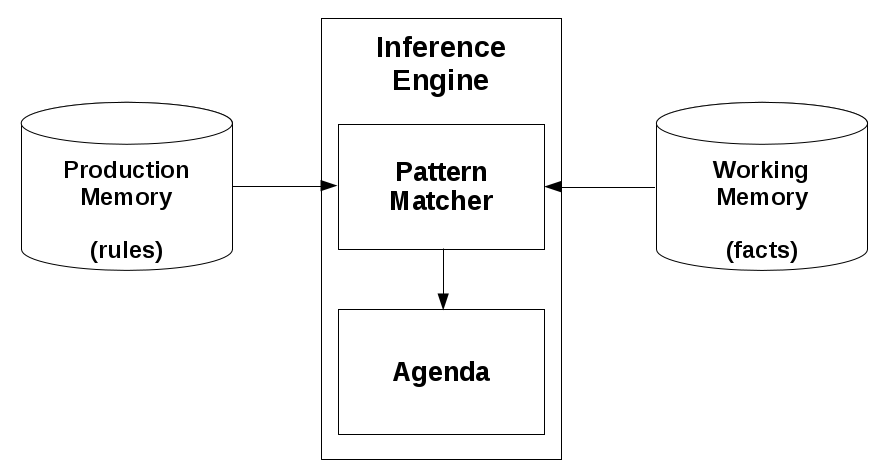
\includegraphics[scale=0.35]{pictures/engine}
  \caption{Architettura di un inference engine.}
\end{figure}


\section{L'algoritmo di matching}
Il modulo di matching del sistema si basa sull'implementazione dell'algoritmo RETE. Per la sua efficienza, rappresenta un punto d'inizio per ricerche, miglioramenti e discussioni nell'ambito dello sviluppo di un motore inferenziale. Il concetto alla base di RETE è quello della scomposizione atomica di tutte le parti sinistre delle regole e della costruzione di un grafo per la verifica di un singolo fatto in una prima fase e successivamente di più fatti congiunti da uno o più predicati.
I punti di forza di questo algoritmo sono:
\begin{itemize}
\item L'\textbf{utilizzo di memorie} (alfa e beta) contenenti riscontri parziali, le quali permettono di ridurre il numero di controlli effettuando un match solo su un nuovo fatto asserito, senza verificare nuovamente i fatti già presenti nella working memory.
\item La \textbf{condivisione dei nodi} tra regole di produzione che hanno stesse condizioni in comune sia nell'alfa network che nella beta. In TURTLE, attualmente, la condivisione dei nodi avviene solamente nell'alfa network; ciò comporta una duplicazione di nodi nella beta network. 
\end{itemize}

RETE presenta anche alcuni svantaggi che naturalmente coinvolgono anche l'algoritmo di matching realizzato per TURTLE:
\begin{itemize}
	\item Si verificano \textbf{sprechi di memoria} dovuti alla duplicazione di riferimenti ai token (nonché ai wme) nelle beta memory.
	\item L'\textbf{eliminazione} di uno o più fatti rappresenta un'operazione non banale all'interno del grafo poiché andrebbero rimossi tutti i riferimenti ed i token generati in cui tali fatti compaiono (operazione denominata retract).
	\item Spesso si verificano \textbf{propagazioni nulle} tra i nodi beta che non avranno mai un'attivazione destra (o solo pochi di essi andranno avanti). Tale problema viene definito ``\emph{utility problem}''\cite{minton1990quantitative}.
		\item Le \textbf{performance} possono diventare drastiche se le condizioni nelle regole sono definite in un ordine sparso, con test ridondanti ed eccessive ritrattazioni.
\end{itemize}

Nella definizione di matching rientra esclusivamente l'algoritmo che viene eseguito quando si verificano attivazioni destre e sinistre. Tuttavia, per permettere tali operazioni e renderle meno costose, esiste una fase di costruzione e definizione delle strutture, pronte per essere attraversate in fase di matching. Per cui, è necessario distinguere la fase di \textbf{build} da quella di \textbf{match}: la prima viene eseguita subito dopo il parsing e l'interpretazione del file, costruendo la rete (alfa e beta), distribuendo i test nei punti opportuni e collegando i pattern di una medesima produzione tra di loro; la seconda, invece, attraversa i suddetti nodi, esegue i test nei nodi che prevedono determinati controlli ed infine costruisce e propaga dei record di fatti denominati \emph{token}.

\subsection{Alfa Network}
La parte alfa della rete è composta da un nodo radice (\textbf{root node}), da nodi alfa (\textbf{alfa node}) e da nodi di memoria (\textbf{alfa memory}).

\subsubsection{Fase di costruzione}
La \textbf{costruzione} dell'\emph{alfa network} avviene in avanti partendo da un nodo radice fino a raggiungere i nodi delle memorie alfa.

Dopo aver costruito un \emph{nodo radice}, si collegano ad esso i \emph{nodi alfa} che rappresentano il nome di ciascun pattern. Ad ogni diramazione corrisponde la scomposizione di un pattern. Se due o più pattern aventi lo stesso nome presentano gli stessi campi a partire dal primo, allora condividono tutti i nodi in comune fino a quanto non presentano campi diversi. I nodi terminali, cioè i nodi foglia, di ciascuna diramazione dell'alfa network sono dei \emph{nodi alfa memory}, nei quali vengono memorizzati i \emph{WME} riconosciuti dalla rete alfa.

L'alfa network è costruita mediante la chiamata di un metodo di \textbf{build}, presente nelle classi che rappresentano i nodi di tale rete. A ciascun nodo è delegata la costruzione del nodo successivo e la chiamata del metodo di build del nodo appena costruito. I nodi rappresentano i propri figli mediante dizionari di nodi indicizzati rispetto all'etichetta che ne rappresenta il campo corrispondente. La scelta del dizionario per la rappresentazione dei figli di un nodo è dettata dalla necessità di dover individuare immediatamente, durante la fase di build, la necessità di condividere o no un nodo e, durante la fase di \textbf{match}, il nodo corrispondente al successivo valore di un fatto. Il modello di riferimento è stato quello della \emph{Data Network with Hashing}\footnote{\url{http://reports-archive.adm.cs.cmu.edu/anon/1995/CMU-CS-95-113.pdf}}.

Il metodo di build del \emph{root node} riceve in input un pattern e costruisce un figlio di tipo \emph{alfa node} o ne condivide uno già esistente, a seconda che il nodo abbia o no un figlio con l'etichetta corrispondente al primo elemento di tale pattern; in seguito tale metodo richiama il metodo di build del nodo appena costruito.

Il metodo di build della classe \emph{alfa node} riceve in input un pattern e un dizionario, inizialmente vuoto, delle variabili incontrate durante la scansione del pattern. Il metodo in questione memorizza nel nodo corrente un valore di profondità, che indica la posizione, incrementata di una unità, del campo del pattern che si sta considerando, in modo da facilitare la successiva fase di match, dato che si stabilisce una corrispondenza uno-ad-uno tra campo del pattern e campo di un fatto. Il valore di profondità è uguale a 0 per il primo campo successivo al nome del pattern, ovvero per il primo livello di nodi alfa costruiti. Il metodo di build dei nodi alfa, in modo analogo a quanto detto per il nodo radice, costruisce un figlio, dato da un altro nodo alfa, o ne condivide uno esistente, a seconda che il nodo abbia o no un figlio con l'etichetta corrispondente al campo che si sta considerando; in seguito si richiama il metodo di build del nodo appena costruito.

La rappresentazione dei nodi alfa prevede, oltre al dizionario di figli indicizzati per campo e al valore che indica la profondità di tali nodi, anche l'etichetta dei nodi in questione, un insieme di riferimenti ai figli che corrispondono per eventuali variabili, fondamentale per evitare l'iterazione su nodi che rappresentano costanti durante il match di variabili, e un riferimento all'ultima variabile, se presente, con il nome analogo all'eventuale nome di variabile del nodo corrente, utile ai fini del controllo di uguaglianza in caso di variabili duplicate in uno stesso pattern.

Nel caso in cui si sia giunti alla costruzione dell'ultimo nodo dell'alfa network per il pattern corrente, allora si costruisce un nodo di tipo alfa memory, collegato al nodo corrente, e si richiama il metodo di build di tale nodo, il quale restituisce un riferimento a se stesso, che verrà propagato lungo le chiamate precedenti, finché non viene restituito a ritroso fino alla chiamata del metodo di build del nodo radice. Ciò permette la memorizzazione del riferimento di ciascuna memoria alfa dell'alfa network, ai fini del collegamento della beta network all'alfa network.

\subsubsection{Fase di matching}
La fase di \textbf{match} dell'\emph{alfa network} è effettuata mediante la chiamata di un metodo di \textbf{match} presente nelle classi che rappresentano i nodi di tale rete. Il metodo di match riceve in input un WME e verifica se, nel dizionario dei figli del nodo corrente, vi è un nodo con etichetta uguale al campo corrente del WME, individuato mediante l'attributo locale di profondità costruito in fase di build: in tal caso si richiama il metodo di match del figlio corrispondente. Se il nodo corrente è stato etichettato come duplicato di una variabile precedente, allora si sfrutta tale riferimento per il controllo dei duplicati. Nel caso in cui l'insieme di riferimenti ad eventuali figli che rappresentano variabili, allora si richiama il metodo di match di tali nodi. Se è stata raggiunta la fine del pattern, e quindi se la fase di match per il WME corrente abbia avuto esito positivo fino al termine dell'alfa network, allora si richiama il metodo di \textbf{attivazione della beta network} presente nella memoria alfa associata al nodo terminale.

Il metodo di attivazione della beta network, presente ne nodi che rappresentano le memorie alfa, prevede la memorizzazione del WME ricevuto in input nella memoria interna del nodo costituita da un dizionario ordinato di WME indicizzate rispetto al loro identificativo numerico (tale struttura dati consente una facile rimozione delle WME durante eventuali operazioni di ritrattazione). Vengono inoltre memorizzate le istanze delle variabili identificate all'interno del pattern che ha superato la fase di match. Si richiama a quel punto il metodo di attivazione del \textbf{match} della \textbf{beta network}.

\subsection{Beta Network}
La parte beta della rete è composta da nodi di join (\textbf{join node} e \textbf{dummy join node}), nodi di memoria (\textbf{beta memory}) e da nodi di tipo production (\textbf{pnode}).

\subsubsection{Fase di costruzione}
La costruzione della \emph{beta network} avviene a ritroso partendo da un \emph{production node} fino a raggiungere i nodi terminali rappresentati dalle memorie della rete alfa già generate.

Partendo da una regola, si scandisce ciascun pattern (test esclusi), si genera un nodo di join associando a quest'ultimo, come input destro, la memoria alfa del pattern; si crea un nodo di memoria beta per l'input sinistro e si ripetono scansione e costruzione sul pattern successivo fino al termine della scansione della parte sinistra di una regola.
L'ultimo pattern letto è associato ad una memoria alfa tramite un nodo dummy join.

Nel caso in cui una regola sia composta esclusivamente da un singolo pattern, viene stabilito un link diretto al \emph{production node}, il quale, nella fattispecie, si occuperà di verificare ciascun WME in arrivo dalla memoria alfa associata ed eventualmente provvederà a far scattare l'attivazione della regola di riferimento. 

Durante la costruzione della rete, se un pattern è nella forma di un \emph{assigned pattern ce}, allora si memorizza nel nodo di join il rifermento alla variabile che conterrà l'istanza di un pattern.

Inoltre, si memorizzano i test che coinvolgono le variabili di ciascun pattern all'interno del nodo di join di competenza: in fase di matching, in seguito al binding delle variabili, verranno eseguiti i test per verificarne il contenuto.

I test e le variabili si possono trovare anche in un production node qualora esista un collegamento diretto ad una memoria alfa.

L'implementazione delle memorie beta è stata realizzata utilizzando dizionari ordinati, i quali permettono un ritrovamento in un tempo ridotto rispetto ad una lista, mantenendo l'ordine di arrivo dei token. Ciò favorisce una riduzione dei tempi in fase di \emph{retract}. Per ciò che concerne le variabili, invece, esse sono memorizzate in dizionari nella forma etichetta-valore.


\subsubsection{Fase di matching}
Quando un WME arriva in una memoria alfa, esso è pronto per essere propagato attraverso la beta network.

Un nodo \emph{beta memory} contiene istanze parziali di regole di produzione, cioè combinazioni di WME che soddisfano in parte una o più regole, cosiddetti \textbf{token}.

Un nodo \emph{join node} ha \emph{due input}: uno \emph{sinistro} a cui è associata una memoria beta ed uno \emph{destro}, a cui è connessa una memoria alfa. Ogni nodo di join si occupa sia di effettuare il binding delle variabili, in comune e non, tra condizioni diverse, che di effettuare i test sugli input ricevuti. L'input sinistro è rappresentato da un token in arrivo dalla memoria beta mentre quello destro è dato da un WME proveniente dalla memoria alfa.

Il binding delle variabili in comune consiste nel verificare che, tutte quelle aventi lo stesso nome, sia nel token che nel WME considerati, abbiano anche lo stesso valore.

Quando un token giunge in un nodo join si parla di \textbf{attivazione sinistra} mentre l'arrivo di un WME fa scattare un'\textbf{attivazione destra}; le attivazioni non possono verificarsi contemporaneamente ed il processo di matching non procede finché non abbiano luogo entrambe: un'attivazione deve attendere il verificarsi dell'altra per poter proseguire la fase di matching.

Se esistono input validi da sinistra e da destra, allora il nodo join si occupa di generare un nuovo elemento unendo i due input in un nuovo token da inviare alla beta memory figlia.
Un caso speciale è rappresentato dal nodo di tipo dummy join che possiede un solo input al quale è associata una memoria alfa (input destro): quando un WME supera il matching nell'alfa network, viene incapsulato in un nuovo token dal dummy join ed il matching prosegue. Il matching in un nodo di join è descritto negli algoritmi \ref{alg:leftactivation} e \ref{alg:rightactivation}.

Le memorie beta ed alfa permettono di riconsiderare rispettivamente token e WME respinti precedentemente, quando certe condizioni sono soddisfatte, con il vantaggio di evitare la ripetizione della fase di matching per ognuno di essi.

Se un token giunge in un \textbf{production node}, allora tutte le condizioni della regola rappresentata dal nodo sono soddisfatte e scatta l'attivazione di quest'ultima; l'insieme delle azioni, presenti nella parte destra della regola, viene aggiunto al conflict set. Il nodo che rappresenta una produzione viene  raggiunto in ultima istanza, per cui rappresenta un nodo terminale. Nelle figure \ref{fig:beta} e \ref{fig:beta1} si possono osservare esempi di matching.

Ogni volta che avviene una propagazione da un nodo di join, vengono generati un nuovo token ed un nuovo dizionario di variabili, unendo le variabili del token considerato con quelle del WME considerato.

\begin{figure}[!ht]
\centering
\begin{verbatim}

		Regole:            Fatti:
		
		    (R1 (f1 ?x)      (fl e1)
		        (f2 ?x)      (f2 e1)
		       ==>....)      (f1 e2)
		                     (f2 e2)
		                     
		Rete:
		             +----------+
		             |   ROOT   |
		             +----------+
		               /      \      		       
		              /        \        
		             /          \        
		        +--------+   +--------+	
		        |   f1   |   |   f2   |   
		        +--------+   +--------+
		            \            /		     
		             \          /
		              \        /
		    x          \      / 
		    =           \    /
		    e1        +--------+ 
		    e2        |  JOIN  |
		              +--------+
		                  | 
		                  |
		                  R1   per x = e1: (f1 e1), (f2 e1)
		                       per x = e2: (f1 e2), (f2 e2)

\end{verbatim}
\caption{Esempio di matching.}
\label{fig:beta1}
\end{figure}

Come già accennato, la fase di ritrattazione di fatti dalla Working Memory implica la cancellazione di tutte le occorrenze dei WME relativi dalla rete, nonché di tutti token in cui tali WME sono presenti. Un token o un WME, quindi, viene eliminato solo quando è eseguita un'azione di \textbf{retract}, altrimenti resta nelle memorie dove occorre, in attesa di partecipare ad un nuovo match.

\begin{algorithm}[h]
 %\SetAlgoLined
 \KwDati{token}
 \KwRisult{new token}
 \Sea{esistono WME nella memoria alfa}{
 	determina le variabili in comune tra le memorie alfa e beta\;
 	\PerCiascun{WME}{
		confronta le istanze delle variabili nel WME rispetto al token\;
		\Sea{il matching va a buon fine}{
			fondi le variabili delle memorie alfa e beta\;
			esegui i test\;
				\Sea{i test sono andati a buon fine}{
					recupera i pattern assignment per il token in input\;
					costruisci un nuovo token Token(token in input, WME corrente)\;
					propaga ai figli del nodo il nuovo token generato, le variabili ed i pattern assignment\;
				}
		}
 	}
 }
 
\caption{Beta network - Attivazione sinistra di un nodo join.}
\label{alg:leftactivation}
\end{algorithm}


\begin{algorithm}[h]
 %\SetAlgoLined
 \KwDati{WME}
 \KwRisult{new token}
 \Sea{esistono token nella memoria beta}{
 	determina le variabili in comune tra le memorie alfa e beta\;
 	\PerCiascun{token}{
		confronta le istanze delle variabili nel token rispetto al WME\;
		\Sea{il matching va a buon fine}{
			fondi le variabili delle memorie alfa e beta\;
			esegui i test\;
				\Sea{i test sono andati a buon fine}{
					recupera i pattern assignment per il token corrente\;
					costruisci un nuovo token Token(token corrente, WME in input)\;
					propaga ai figli del nodo il nuovo token generato, le variabili ed i pattern assignment\;
				}
		}
 	}
 }
 
\caption{Beta network - Attivazione destra di un nodo join.}
\label{alg:rightactivation}
\end{algorithm}

\newpage
\begin{figure}[!ht]
    \vspace*{-2cm}
    \makebox[\linewidth]{
      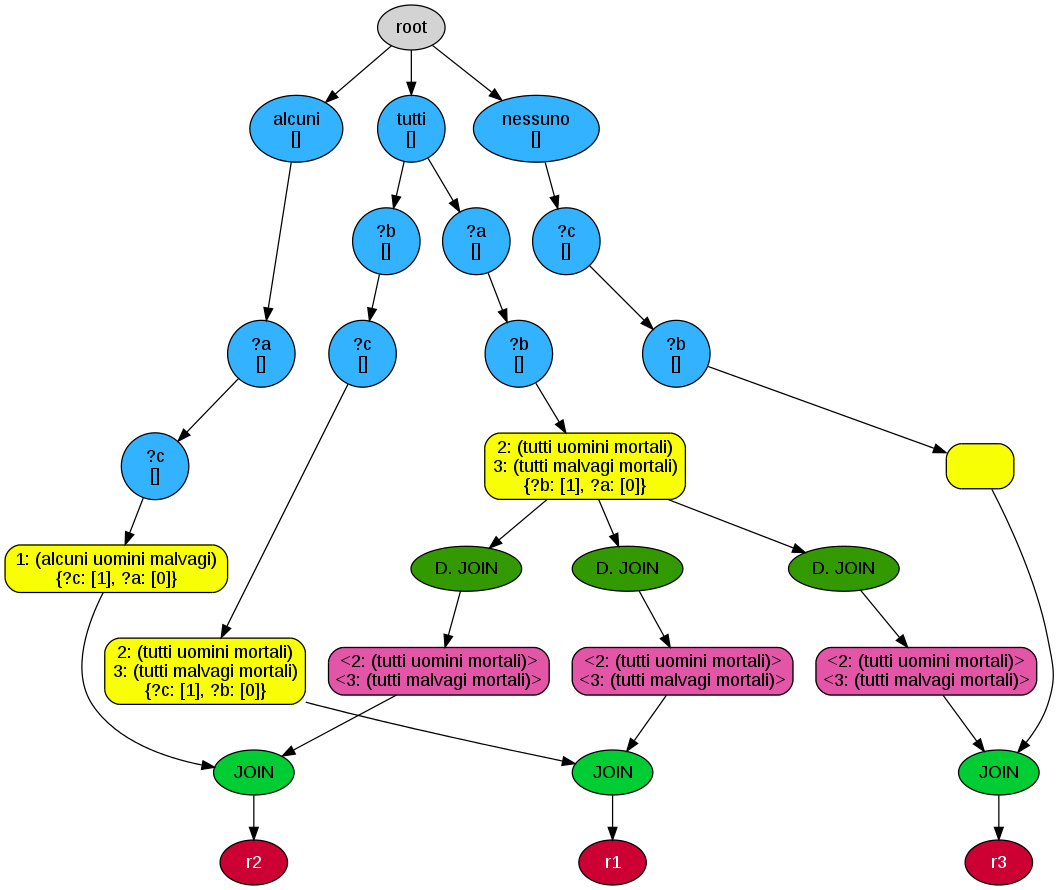
\includegraphics[width=1.4\linewidth]{pictures/beta}
    }
    \caption{Matching beta network per il programma Sillogismi.clp presente nell'appendice di questo documento.}
   \label{fig:beta}
\end{figure}

\newpage
\section{Risoluzione dei conflitti}
Al termine della fase di matching, viene generata un insieme di regole attivabili le cui condizioni sono soddisfatte dai fatti all'interno della Working Memory. Tale insieme prende il nome di \emph{Conflict Set}. Dal momento che il sistema è ispirato a CLIPS, il conflict set prende il nome di \emph{Agenda}. Il fine dell'insieme determinato è quello di risolvere i conflitti tra le regole attivabili selezionandone una ed eseguendone le azioni presenti nella parte destra. La scelta della regola da applicare è effettuata mediante strategie di risoluzione dei conflitti, le quali ordinano le regole applicabili considerandone le proprietà intrinseche e il loro valore di priorità, che prende il nome di \emph{salience}. Dopo l'ordinamento delle regole viene applicata la prima della lista.


L'agenda implementata in TURTLE è composta da un dizionario che associa le salience delle regole attivabili con le liste delle regole aventi tale salience e da un dizionario che associa a ciascun token il numero di regole che esso attiva. L'agenda, inoltre, tiene traccia della strategia scelta e ne permette il cambiamento.


In TURTLE sono state realizzate le seguenti strategie:
\begin{itemize}
\item\textbf{Depth}: È la strategia, come in CLIPS, di \textbf{default}. Tale strategia ordina le regole attivabili in base al loro tempo di attivazione: le regole attivate dal fatto più recente vengono posizionate al di sopra delle regole aventi la stessa salience attivate dai fatti meno recenti. La strategia in questione è denominata depth poiché è una depth-first-search.
\item\textbf{Breadth}: Le regole attivate dal fatto più recente vengono posizionate al di sotto delle regole aventi la stessa salience attivate dai fatti meno recenti. La strategia in questione è denominata breadth poiché è una breadth-first-search, in cui l'ordine delle attivazioni è gestito come se fosse una coda.
\item\textbf{Random}: Le regole attivabili vengono mescolate in un ordine casuale.
\item\textbf{Simplicity}: Tra tutte le regole con la stessa salience, le nuove attivazioni vengono inserite al di sopra di quelle corrispondenti a regole con uguale o maggiore specificità, definita in base ai seguenti criteri di analisi per la loro parte sinistra:
	\begin{itemize}
	\renewcommand{\labelitemii}{$\cdot$}
	\item\textbf{+1} per ciascun pattern.
	\item\textbf{+1} per ciascuna variabile univoca.
	\item\textbf{+1} per ciascuna funzione o predicato.
	\end{itemize}
\item\textbf{Complexity}: Tra tutte le regole con la stessa salience, le nuove attivazioni vengono inserite al di sopra di quelle corrispondenti a regole con uguale o minore specificità.
\item\textbf{LEX}: È una implementazione Naive della strategia LEX di CLIPS. Le regole attivate dai fatti più recenti vengono posizionate al di sopra delle regole aventi la stessa salience attivate dai fatti meno recenti. Rispetto alla strategia depth la priorità di una regola è data da un ordinamento lessicografico dei fatti che la attivano piuttosto che dall'individuazione del fatto più recente.
\item\textbf{MEA}: È una implementazione Naive della strategia MEA di CLIPS. Le regole in cui il primo fatto dei token che le attivano è più recente vengono posizionate al di sopra di quelle in cui il primo fatto dei token che le attivano è meno recente.
\end{itemize}

\newpage
\section{La shell d'interazione}
Per caricare un programma, eseguirlo, ed interagire con esso, è necessario avviare TURTLE da riga di comando\footnote{Sono necessarie alcune dipendenze, specificate in un file di testo nella directory del progetto.}. Il file da passare in input all'interprete Python è \textbf{Turtle.py} (\textbf{python -B Turtle.py})\footnote{Il parametro ``-B'' serve ad evitare la creazione del file .pyc contenente il bytecode; quest'ultimo permette di avviare rapidamente il sistema, ma non offre alcun vantaggio in fase di esecuzione.}.

Dopo aver avviato il sistema, un prompt sarà a disposizione per ricevere i comandi necessari al caricamento e all'esecuzione di un programma a regole, solitamente contenuto in un file di testo con estensione ``.clp''.

\begin{figure}[!ht]
\centering
\begin{verbatim}
                 __
      .,-;-;-,. /'_\  TURTLE Pre-Release
    _/_/_/_|_\_\) /
  '-<_><_><_><_>=/\   An expert system shell inspired by CLIPS syntax
    `/_/====/_/-'\_\  Running on Python 2.7.3 32bit
     ''     ''    ''
    Usage: help to see online help
           <Tab> to show commands
           <Up-arrow>, <Down-arrow> to scroll through the history
           <Ctrl-c> to break a running program
           <Ctrl-d>, quit or exit to leave


TURTLE> 
\end{verbatim}
\caption{Prompt della shell.}
\label{fig:prompt}
\end{figure}

Nella figura \ref{fig:prompt} viene mostrato come si presenta il prompt dei comandi all'avvio del sistema. L'interfaccia testuale propone un banner informativo con le scorciatoie da tastiera ed i comandi utili per interagire, i quali offrono diverse comodità come la possibilità di richiamare comandi già digitati in precedenza, il completamento automatico e l'help online. 

Quest'ultimo fornisce spiegazioni sull'utilizzo di tutti i comandi oltre che le liste di funzioni e predicati disponibili ed utilizzabili all'interno di fatti e regole. E' possibile eseguire un programma impostando un limite d'esecuzione oltre il quale viene fermato il ciclo riconosci-agisci, lasciando in agenda tutte le attivazioni non ancora eseguite.

Per fornire compatibilità sintattica con CLIPS, è possibile racchiudere opzionalmente ogni comando tra parentesi tonde; per cui, ad esempio, il comando \textbf{help} è equivalente al comando \textbf{(help)}.

%\vspace{0.5cm}
%\begin{figure}[!ht]
%  \centering
%  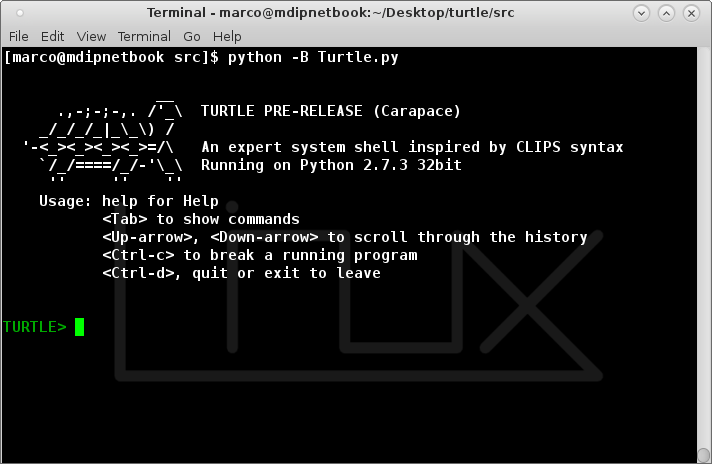
\includegraphics[scale=0.50]{pictures/cmdavvio}
%  \caption{Avvio della shell.}
%  \vspace{0.5cm}
%  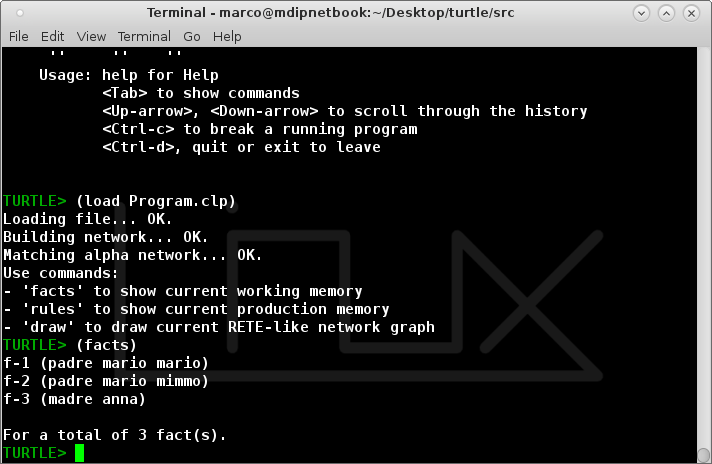
\includegraphics[scale=0.50]{pictures/cmdfacts}
%  \caption{Caricamento di un programma.}
%\end{figure}

La shell dispone del completamento automatico del testo premendo il tasto TAB. Se quest'ultimo viene premuto senza aver digitato alcun carattere, verrà mostrato l'intero elenco dei comandi che è possibile impartire alla shell.

Si possono definire fatti, regole e variabili globali direttamente da shell oltre che caricare uno o più file. Al contrario di CLIPS \footnote{CLIPS, dopo un reset ripristina solo tutti i fatti che sono stati definiti tramite il costrutto deffacts, da shell o da file.}, tutti gli elementi definiti dalla shell tramite \emph{assert} o \emph{deffacts} (oltre quelli caricati da file), dopo un \emph{reset}, saranno mantenuti in memoria. Attualmente la command line non accetta comandi multi-riga.

Se si intende ripulire l'intero ambiente è necessario il comando \emph{clear}, come avviene in CLIPS.
